\subsection{Algorithm process}
Figure \ref{fig:pentos} shows the high level process of our algorithm. It first picks the best valid location to build the requested building, which is chosen based on several criteria. Then, build the best road to connect it to an existing road or edge. If the request is a residence, there is an additional step to build an accompanying park and pond. A detailed illustration will be presented in the next subsection.

\begin{figure}
\center
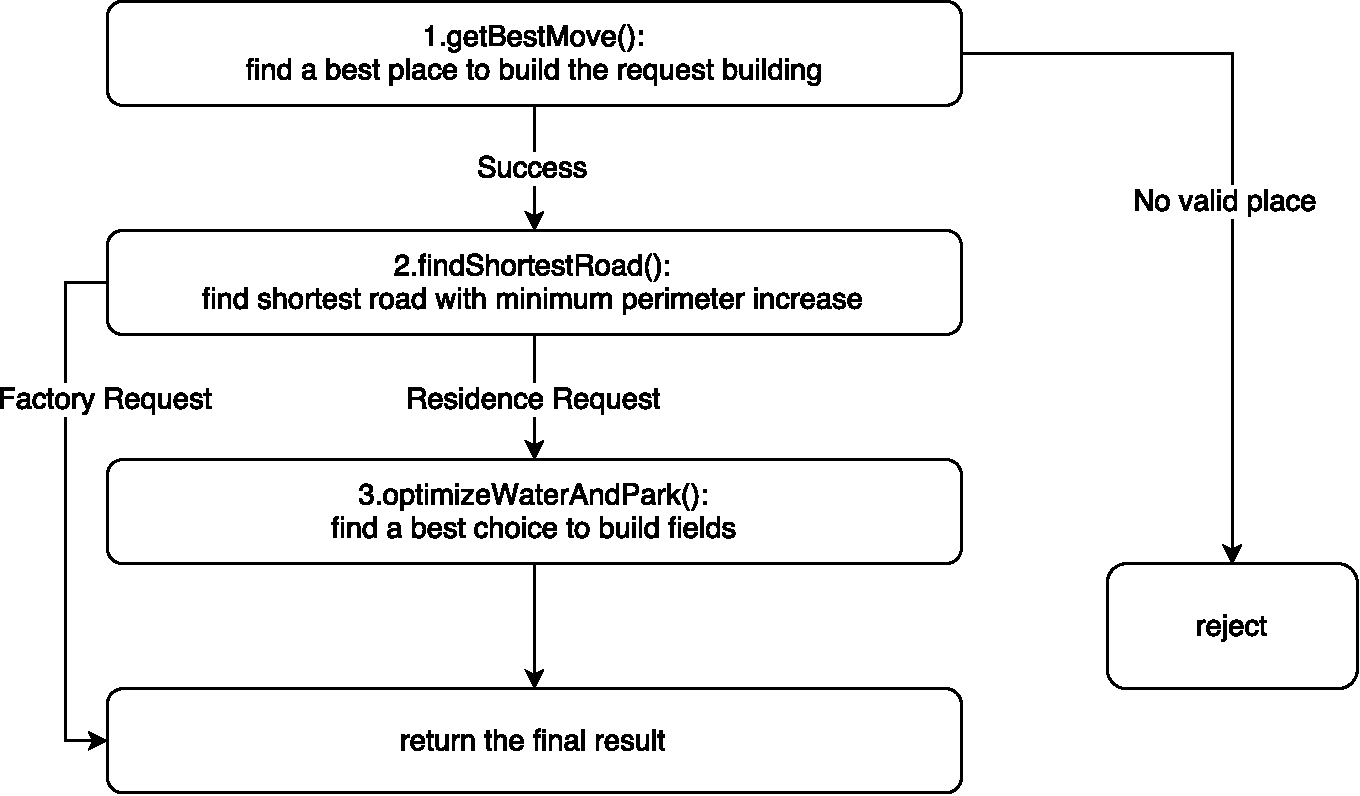
\includegraphics[scale=0.5]{pentos.pdf}
\caption{high level algorithm flow chart of our submitted approach}
\label{fig:pentos}
\end{figure}

\subsection{Building Placement}
The purpose of this module is to find the best place to build the requested building. We look at every possible coordinate that the building could be placed such that it does not overlap with any other buildings, roads, parks or ponds. Then we filter out the coordinates that are in white spaces that are cut off from roads or edges. Then, we try to define the "best" coordinate using different approaches, which will be explained in each of the following sections. \\
We define a global strategy to be the strategy that decides the overall preference of location for the factories and residences, based solely on the value of its coordinates and not on the position of other buildings.

\subsubsection{Pre-allocation}
%\subsubsection{global: row-by-row}
Due to the constraint that residences and factories cannot be adjacent to each other. It's reasonable to keep them away from each other. One of the simplest approach to this idea is, we ``pre-allocate" the residence area and factory area. We give different priorities to the location where the building should be built at for the incoming residence and factory. It doesn't mean that some locations are forbidden for residence/factory construction. Below is a list of strategies we have tried.

\paragraph{Row-by-row construction}
This is a naive strategy that we tried first. The residences are built row by row from the top to bottom, which means that for each residence, iterate over coordinates from the top left to the bottom right each time, finding the first buildable coordinate (which will have the lowest row index). The factories are built row by row from the bottom to the top, which means for each factory, iterate over the rows from the bottom right to top left, finding the first buildable place (which will have the highest row index). The idea behind this approach is to separate the residences and factories. The reason behind this is that factories are rectangular shaped and would fit together well. Similarly, residences being irregular, would not fit with factories. The other reason for separating them is that factories and residences cannot be built adjacent to each other. This means that placing them close to each other would create large white spaces. To avoid this, we build residences at the top and factories at the bottom.

Using this naive approach, we could get a score of around 1600 to 1700, depending on whether or not we used ponds and parks. The implementation of the naive strategy help us more understand the game at the beginning. It also helped us estimate the utility of parks and ponds, since including them increased our score by around 100.\\
Later, we switched to other strategies.

%\subsubsection{global: diagonal}
\paragraph{Building along the diagonal}
This is another strategy of placing residences and factories in a way that separates them from each other. The residences are built from the top left corner to the bottom right corner, which means each time find the buildable coordinate with the lowest sum of row index and column index. The factories are build from the bottom right corner to the top left corner, which means each time find the buildable coordinate with the highest sum of row index and column index.\\

The idea behind this approach is similar to the row-by-row approach in that it tries to separate the residences and factories. However, the diagonal gap is better than the row-by-row strategy because there are a larger number of possible locations with the same $(i+j)$ value to choose from. In addition, using this strategy we can better utilize the four borders but in row-by-row construction two of them are quickly occupied in the beginning.\\

In addition to the global diagonal pattern, we add another small features to the selection process. For the candidate spaces that have the same value of $(i+j)$, which denotes the sum of row index and column index, we pick the one that has the lower value of $|(i-j)|$, which means the one closer to the diagonal line. The idea behind this feature is to make the frontier of residences and factories more convex. Since edges are considered roads, building buildings further from the edges first increased the flexibility of how we use the edges later. In addition, placing a factory near the edge always creates very few white spaces, so if we have an equally good option for the factory away from the edge, it would make sense to pick the option away from the edge and save the edge for a future factory.

%\subsubsection{global: residences at center, factories on edges}
\paragraph{Residences at the center, factories to the borders}
This is a different global strategy we have tried. In this strategy, we build factories from the edges to the center and build residences from the center to the edges like what we are doing in real worlds. 

The idea behind it is that the factories are more regular in shape so they can fit very well on the edges, while residences have more irregular shapes. But the experiments demonstrated to us that this is not a good strategy, so we gave up on it later. 

There are two reasons that we decided to avoid this strategy. The first problem with this is if we build all the factories near the edges, it makes the gap between factories and residences longer. Also there is another problem in that, it is vulnerable to adversarial distributions as it increases the difficulty of building roads. If we get an adversarial distribution that requests factories first, this strategy would build factories around the borders and cut off the inner area from outside. 

\subsubsection{Jigsaw Puzzle approach}
The main idea of our submitted player is that, after placing the requested building, the remain empty region should be ``regular". A square-shaped empty region is more favored since it has more freedom for the future placement. We don't like the border of empty region to be irregular because it may require some special shape to well fit into it. Another bad example is a long-bar-shaped empty region, it restricts the alignment of the building.

Based on this idea, we propose a robust measurement of ``regularity" -- the {\bf perimeter} of all the objects that have been placed.
The perimeter strategy is a non-global strategy that looks at the cells around the candidate location for a requested building. For a candidate location, some of its cells are adjacent to already occupied cells in the map and some of its cells are neighbor to vacant cells in the map. The algorithm count the number of edges of the neighbour that it shares with an occupied cell, which is the perimeter of this location. Then we choose the candidate with the largest perimeter. The idea behind it is the larger perimeter means the buildings are more compactly packed. And, it has been shown that perimeter evaluation made a significant contribution to our good performance. Adding this strategy improved the score of the naive global strategy by around 300 points. 

Finally, we use the diagonal strategy as our global strategy. However, we only use it to break ties between candidates that have the same perimeter.\\

We also tried a different way to count the perimeter. That is to count the number of cells surrounding the candidate location, should the building be placed there. This differs from the the ordinary perimeter strategy, since the previous strategy counts edges instead of cells, so it might count certain cells multiple times. In practice, the edge counting strategy worked better, scoring around 30 points more. The reason for this is described in figure \ref{fig:plusu}.

\begin{figure}
\center

\includegraphics[scale=0.05]{pentomino.jpg}
\caption{If only the number of cells were counted, placing the U pentomino on the plus pentomino would have a score of 3, same as placing it against an edge. Counting edges gives a score of 5 versus the same 3 for an edge}
\label{fig:plusu}
\end{figure}

As a summary, in the submitted version, we use the diagonal global strategy and the perimeter local strategy. When comparing different choices, we use the perimeter as the first key, $(i+j)$ as the second key, and $(i-j)$ as the third key.

\subsubsection{The number of disconnected components}

Based on the ``regularity" ideas before, we have tried another criterion to choose the best location.

In the previous section, we mentioned the number of cells that neighbor to already occupied cell. It generally makes the buildings compact, but sometimes creates small cut off areas that lower the land use efficiency. so we consider another measurement called number of components. It is defined as the number of connected components comprising vacant cells that are created when a building is placed. The idea is to create as few vacant components as possible. Figure \ref{fig: numComponents} shows the idea more intuitively.

\begin{figure}
\center
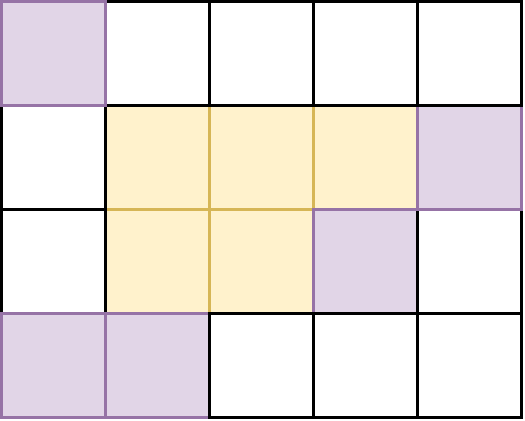
\includegraphics[scale=0.5]{numComponents.pdf}
\caption{
Suppose the yellow grids denote the candidate building place,
the purple grids denote already occupied cells,
the white grids denote vacant cells.
Then the number of components in this example is 3.}
\label{fig: numComponents}
\end{figure}

Sadly in our experiments, we tried using the number of components as either the first or second key, but the score decreased slightly, while significantly slowing down the simulation.

